\chapter{Technologies}
This chapter focuses on the specific technologies utilized in implementing Kube. Foremost among
these is the suite of AWS services, including Lambda for serverless computing, SQS (Simple Queue
Service) and SNS (Simple Notification Service) for messaging, and RDS (Relational Database Service)
for database management. These services collectively provide a resilient and scalable infrastructure
for Kube. Additionally, the platform leverages the serverless architecture to optimize resource
utilization and reduce operational overhead and the Go programming language for its efficiency and
suitability for building high-performance applications. The user interface of Kube is crafted using
Flutter, a versatile UI toolkit, which enhances the platform's accessibility and aesthetic appeal.
Together, these technologies form the cornerstone of Kube, enabling it to deliver good performance
and user experience.

\section{Amazon AWS Services}
AWS is recognized as the world's most comprehensive and broadly adopted cloud platform. It offers
over 175 fully featured services from data centers globally. AWS is utilized by a diverse range of
customers, including rapidly growing startups, large enterprises, and leading government agencies,
to reduce costs, increase agility, and accelerate innovation. The platform provides a wide array of
cloud-based products including compute, storage, databases, analytics, networking, mobile, developer
tools, management tools, IoT, security, and enterprise applications, all available on-demand with
pay-as-you-go pricing\textsuperscript{\cite{tech_1}}. In this section we will analyze the most
important services offered by Amazon AWS that we will use in the development of the project.

\newpage

\subsubsection{Example of AWS services integration}

\begin{figure}
    \centering
    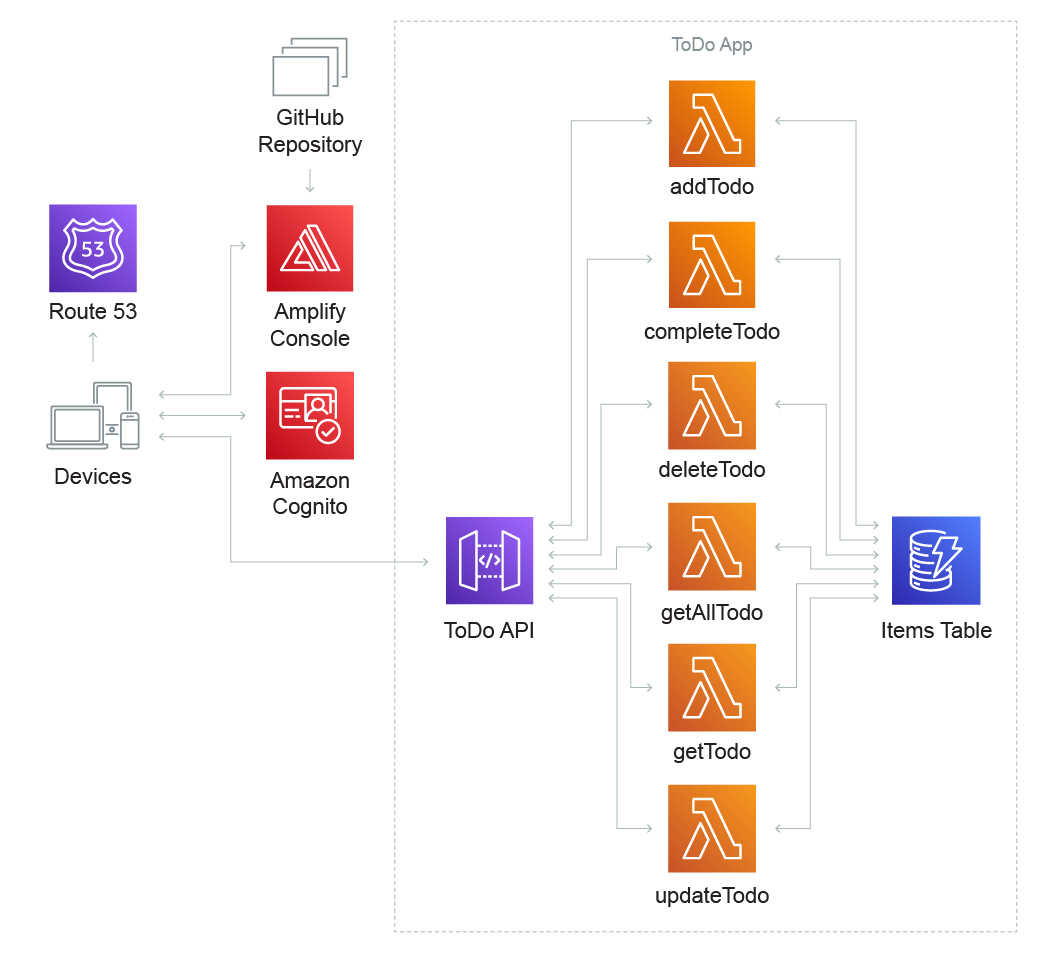
\includegraphics[scale=0.3]{Pictures/3_serverless_example.jpg}
    \caption{Example of AWS services integration.}
    \label{fig:3_aws_example}
\end{figure}

The image \ref{fig:3_aws_example} illustrates the architecture of a simple "to-do list" web
application built using serverless technology on the Amazon public cloud. This event-driven
application is designed to allow registered users to manage their tasks efficiently. Users interact
with the application to create, update, view, and delete to-do items. The architecture integrates
several Amazon Web Services to achieve this functionality. Each component of the architecture is
orchestrated to respond to specific events triggered by user actions, such as adding a new to-do
item or marking one as complete, making the entire application responsive and scalable without the
need to manage server infrastructure\textsuperscript{\cite{serverless_1}}.

\subsection{Pros and cons}
Amazon Web Services (AWS) is renowned for its extensive array of over 200 fully-featured services,
ranging from fundamental infrastructure technologies like compute, storage, and databases to
cutting-edge fields such as machine learning, AI, data lakes, analytics, and IoT. This diversity
offers tailored solutions for different applications, optimizing both cost and performance. However,
the sheer breadth of services can be overwhelming for less experienced users and creates a potential
dependency on AWS, making it challenging to switch providers. Additionally, while AWS allows for
cost and performance flexibility, improper resource management or unsuitable service choices can
lead to high expenses.

\subsection{Alternatives}
Microsoft Azure and Google Cloud Platform (GCP) stand as significant alternatives to Amazon Web
Services. Azure, backed by Microsoft's legacy in enterprise software, excels in integrating with
existing Windows-based environments, making it a preferred choice for organizations deeply embedded
in Microsoft's ecosystem. It offers a strong focus on hybrid cloud, AI, and machine learning
capabilities. On the other hand, GCP is highly regarded for its deep expertise in data analytics,
machine learning, and open source technologies, leveraging Google's pioneering work in these
areas\textsuperscript{\cite{cloud_azure}}\textsuperscript{\cite{cloud_google}}. The table
\ref{fig:3_cloud_comparision} shows a comparison between the major four cloud services providers.

\begin{figure}
    \centering
    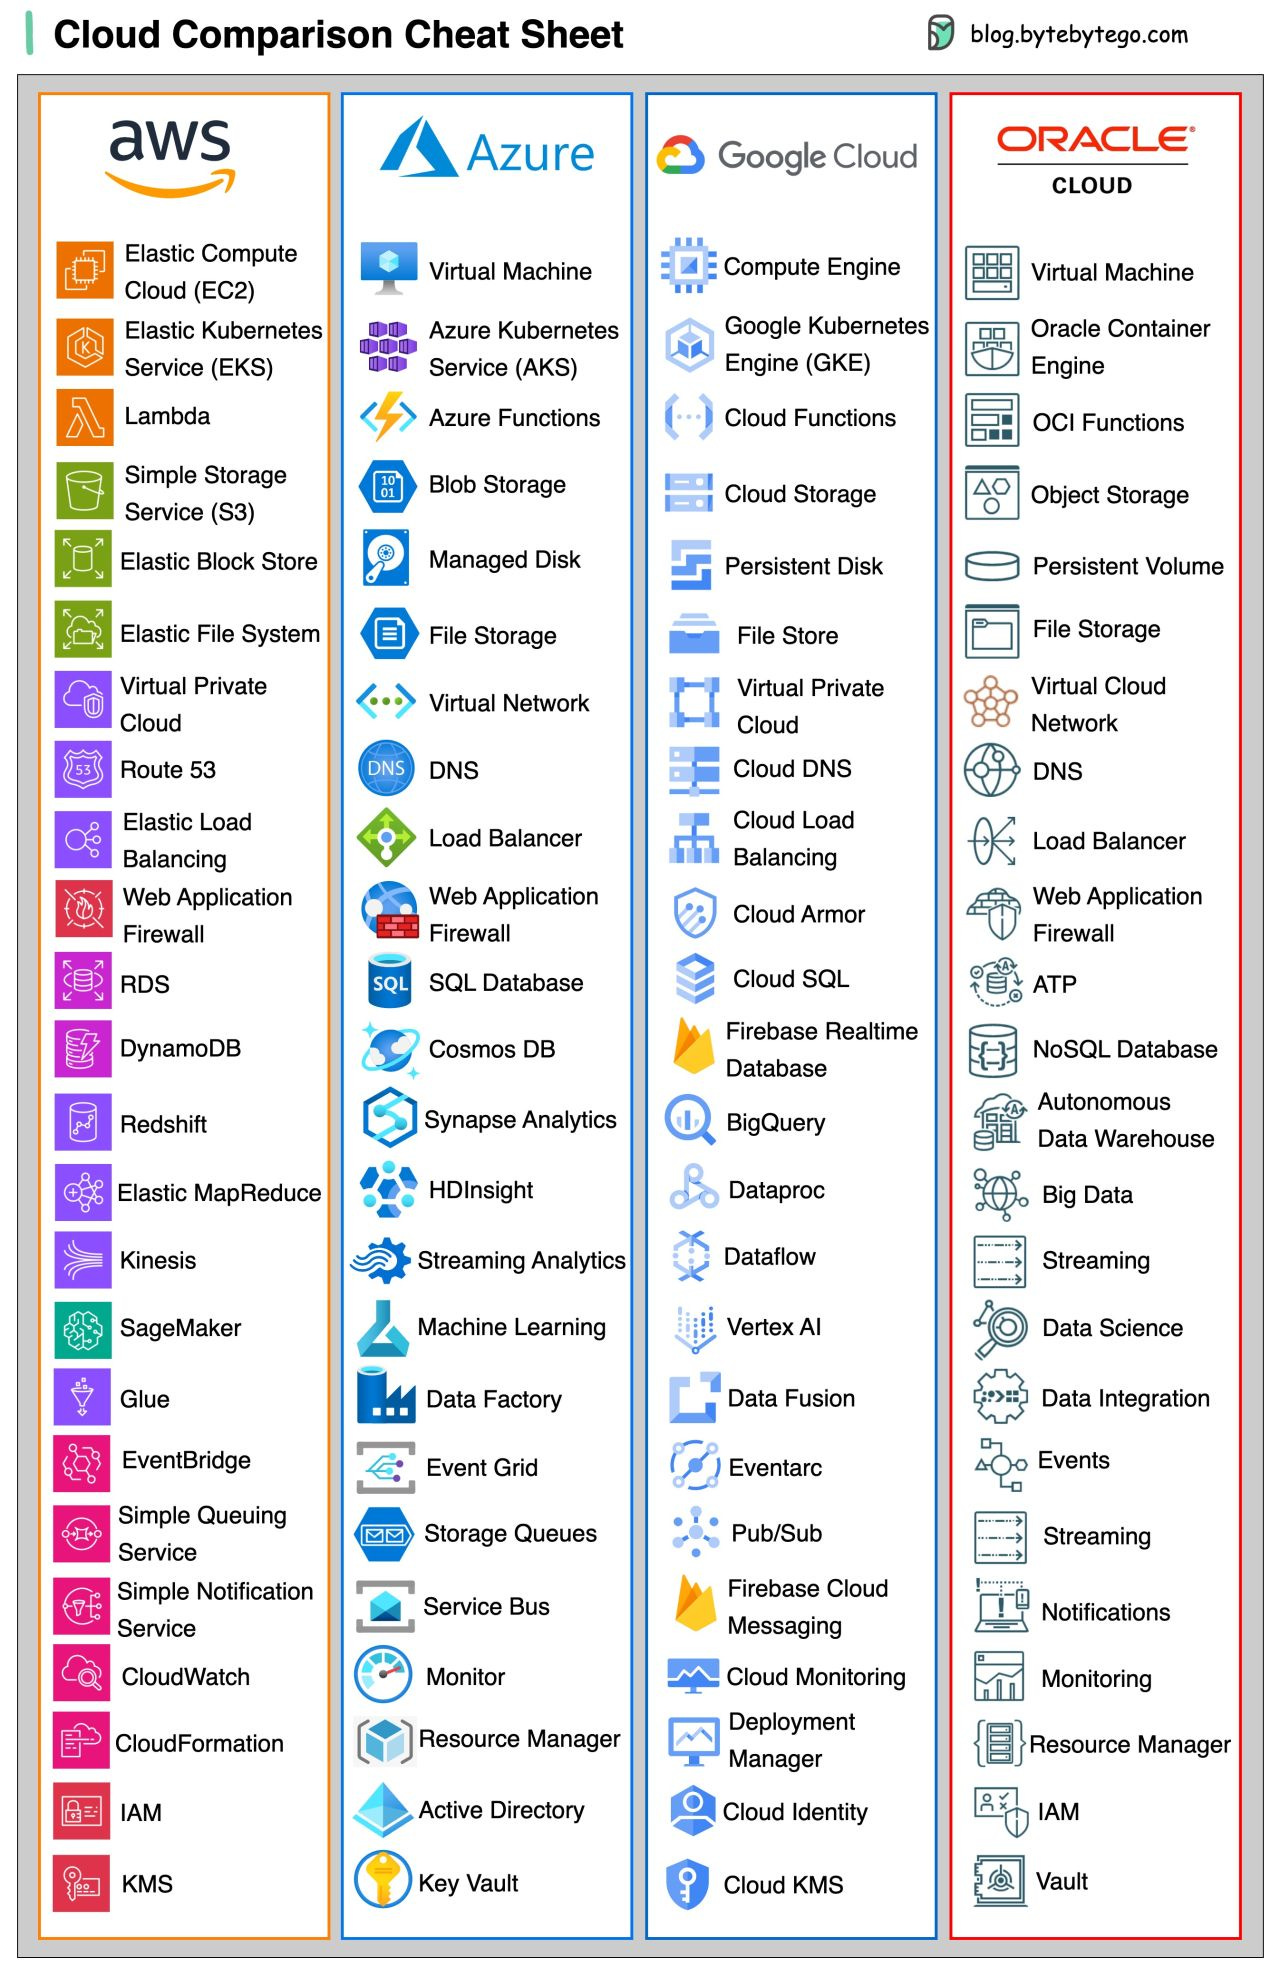
\includegraphics[scale=0.18]{Pictures/3_cloud_comparision.jpg}
    \caption{Cloud services comparison\textsuperscript{\cite{tech_8}}.}
    \label{fig:3_cloud_comparision}
\end{figure}

\subsection{AWS API Gateway}
Amazon API Gateway is a fully managed service that simplifies the creation and maintenance of APIs,
serving as the gateway for applications to access backend data and services. It supports various
workloads, including real-time communication through RESTful or WebSocket APIs, and handles tasks
like traffic management, security, and monitoring. Plus, there are no upfront fees, and you pay
based on your API usage, with pricing that scales according to your
needs\textsuperscript{\cite{tech_2}}.

\subsection{AWS Lambda}
AWS Lambda is a serverless computing service from Amazon Web Services, designed to run code without
server provisioning or management. It executes code in a high-availability environment, handling all
aspects of computational resource administration. This approach allows for code organization into
Lambda functions, which are executed and automatically scaled as needed, with billing based on
compute time used. Ideal for scenarios requiring rapid scaling, Lambda supports diverse applications
like real-time data processing with Amazon S3, streaming data handling with Amazon Kinesis, and
creating scalable web and serverless back-ends for IoT and mobile devices. Key features include easy
function configuration, environment variables, version management, container image support,
packaging libraries, monitoring tools, HTTP(S) endpoints, streaming responses, and code signing for
security. Lambda's flexibility, scalability, and cost-effectiveness make it an attractive solution
for various cloud computing needs, emphasizing efficiency and developer
focus\textsuperscript{\cite{tech_3}}.
\newline\newline
AWS Lambda functions can be invoked in various ways, depending on the needs of the application. One
common method is through event triggers, which can include changes in data within AWS services like
S3 bucket updates or DynamoDB table updates. These events can be configured to invoke a Lambda
function synchronously or asynchronously how showed in figure \ref{fig:3_lambda_invocation}.

\begin{figure}
    \centering
    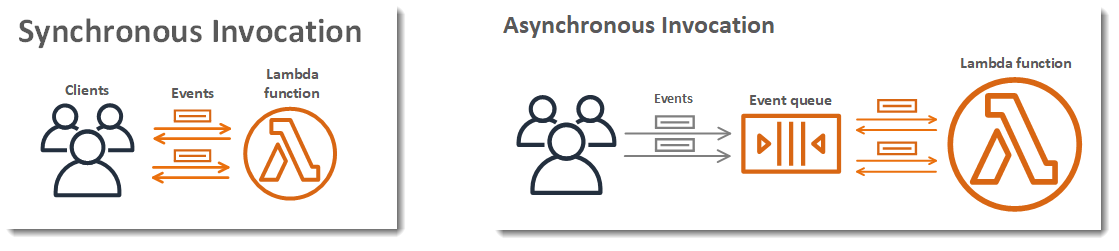
\includegraphics[scale=0.5]{Pictures/3_lambda.png}
    \caption{Lambda invocation types.}
    \label{fig:3_lambda_invocation}
\end{figure}

Synchronous invocation, where the caller waits for the function to process the event and return a
response, is commonly used in scenarios like API executions through Amazon API Gateway. Asynchronous
invocation is employed when the order of execution is not critical. In this case, events are placed
in a queue before being sent to the function, and AWS Lambda manages the function's invocation rate.
For asynchronous execution, AWS also provides services like Amazon Simple Queue Service (SQS) for
queueing messages or Amazon Simple Notification Service (SNS) for delivering messages to subscribing
endpoints or functions. These services can be directly integrated with Lambda to handle
event-driven, scalable computing architectures, allowing developers to focus on code rather than
infrastructure management.

\subsection{AWS RDS}
Amazon Relational Database Service (Amazon RDS) is a web service from AWS that simplifies setting
up, using, and scaling relational databases in the cloud. It offers scalable, cost-effective
solutions for standard industry relational databases, managing common administrative tasks, thus
allowing users to focus more on their applications and user engagement. As a fully managed service,
Amazon RDS handles the majority of management tasks, relieving users from manual and time-consuming
database maintenance. It supports various popular database engines, such as Amazon Aurora, MySQL,
MariaDB, PostgreSQL, Oracle, and SQL Server. Additionally, Amazon RDS provides deployment
flexibility, including on-premises options with Amazon RDS on AWS Outposts. This combination of
versatile database engine support, automated management, and deployment options make Amazon RDS a
comprehensive and user-friendly solution for managing relational databases in the AWS
Cloud\textsuperscript{\cite{tech_4}}.

\subsubsection{RDS vs DynamoDB}
AWS does not offer only SQL options with RDS; there is also DynamoDB, a NoSQL alternative for
different database needs. While RDS excels in structured data management and complex querying
capabilities via SQL, DynamoDB provides a flexible schema with key-value and document data models,
delivering quick and predictable performance. RDS is preferable for traditional applications that
need transactional support, complex joins, and other SQL operations. In contrast, DynamoDB is
tailored for modern applications that demand scalability, low-latency data access, and where
database management overhead should be minimized. The choice between RDS and DynamoDB hinges on the
application's data requirements and scalability demands.

\subsection{AWS SQS}
Amazon Simple Queue Service (SQS) is a fully managed message queuing service for microservices,
distributed systems, and serverless applications, offering secure and reliable data transfer without
losing messages or depending on other services' availability. Amazon SQS provides key benefits such
as security, with user-controlled access and server-side encryption options using AWS Key Management
Service, and durability, ensuring message storage across multiple servers. Its high availability is
maintained through a redundant infrastructure for consistent message access. The service is highly
scalable, processing each request independently to manage load spikes, and guarantees reliability by
locking messages during processing to support multiple producers and consumers. Amazon SQS also
allows for customization, like setting default delays on queues or storing large message contents on
Amazon S3 or DynamoDB. These features make Amazon SQS an efficient and versatile tool for handling
large volumes of messages in various application architectures, offering a combination of
reliability, scalability, security, and customization\textsuperscript{\cite{tech_5}}.

\subsection{AWS SNS}
Amazon Simple Notification Service (Amazon SNS) is a fully managed service offering effective
Pub/Sub messaging for both application-to-application (A2A) and application-to-person (A2P)
communication. It facilitates high-throughput, push-based messaging among distributed systems,
microservices, and serverless applications, integrating seamlessly with Amazon SQS, AWS Lambda, and
other services. A2P messaging extends capabilities to customer communications through SMS, push
notifications, and emails. Amazon SNS stands out for simplifying messaging architectures while
reducing costs through features like message filtering, batching, ordering, and deduplication. It
also enhances message durability with storage, delivery retries, and dead-letter queues.
Additionally, it supports strict FIFO message delivery, ensuring accuracy and consistency across
applications. This combination of features makes Amazon SNS a versatile tool for a wide range of
messaging scenarios, from system integration to direct customer
engagement\textsuperscript{\cite{tech_6}}.

\subsection{AWS Cognito}
Amazon Cognito is a comprehensive service designed to implement secure, frictionless customer
identity and access management (CIAM) in a scalable manner. With Amazon Cognito, you can offer a
smooth management of customer identity and access, thanks to its affordable and customizable
platform. It includes features such as adaptive authentication, support for compliance, and data
residency requirements.Amazon Cognito is capable of scaling to millions of users with a fully
managed, high-performance, and reliable identity store. It also provides access to federation using
OpenID Connect (OIDC) or SAML 2.0 and integrates with a broad range of AWS services and products.
This platform supports up to 50,000 active users per month for free under the AWS free tier plan,
making it a cost-effective solution for businesses of varying sizes\textsuperscript{\cite{tech_7}}.

\section{Firebase Cloud Messaging}
Firebase Cloud Messaging (FCM)\textsuperscript{\cite{tech_9}} is a powerful cloud solution for
messages on iOS, Android, and web applications for free. It provides a reliable and efficient
connection between servers and devices that allows for the delivery of notifications or messages.
FCM offers versatile messaging options including topic messaging, which allows you to send a message
to multiple devices that have opted in to a particular topic, device group messaging, allowing for
messages to devices that belong to a group, and direct messaging to individual devices. This
scalability makes it an essential tool for developers looking to engage their user base effectively,
with the added benefits of analytics and performance tracking.

\subsection{How it works}
Firebase Cloud Messaging employs a client-server architecture where the FCM backend is responsible
for handling and routing messages. The client app on a user's device communicates with the FCM via
an SDK, which manages the registration process and token generation. This token uniquely identifies
the app instance and enables secure message delivery to the device. Messages sent from the
developer's server to the FCM backend can be payload-specific, directing the FCM to deliver them as
notification or data messages. FCM then optimizes message delivery by queuing them, managing
priority, and even aggregating messages for network efficiency. This architecture supports a high
level of scalability and reliability in delivering messages across platforms and devices globally.

\begin{figure}
    \centering
    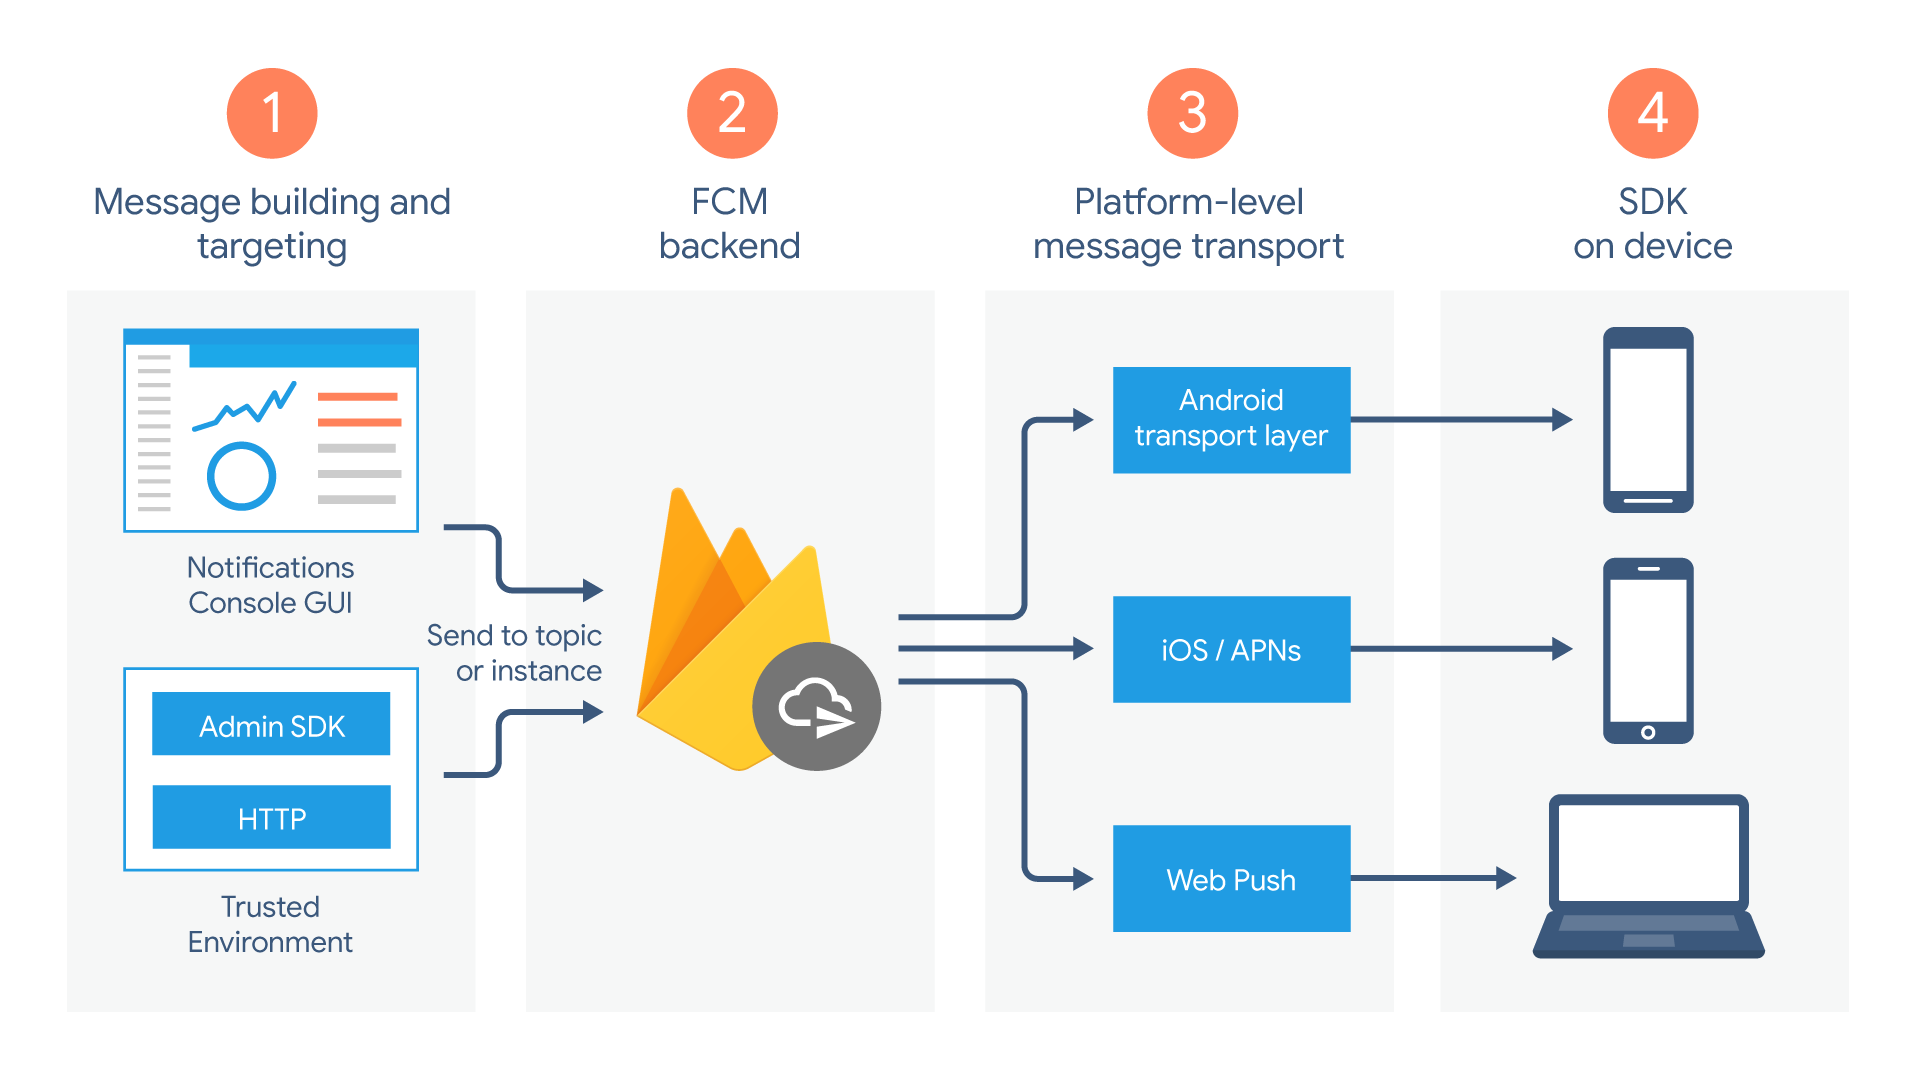
\includegraphics[scale=0.2]{Pictures/3_firebase.png}
    \caption{FCM architecture.}
    \label{fig:3_firebase}
\end{figure}

The image \ref{fig:3_firebase} show the FCM's operational architecture:

\begin{enumerate}
    \item Tools for crafting message requests, including a GUI via the Notifications composer for
          notifications, and server environments like Cloud Functions for Firebase or App Engine,
          supported by the Firebase Admin SDK or FCM server protocol, for comprehensive message type
          handling.
    \item The central FCM server that handles incoming message requests, manages topic-based message
          distribution, and assigns metadata like message IDs.
    \item A device-level transport system that ensures messages reach their destination, varying by
          platform: Android devices, Apple devices and Web push protocols for browsers
    \item The FCM SDK, which resides on the end-user's device, and is responsible for displaying
          notifications or processing messages, depending on the app's state and custom logic.
\end{enumerate}

\section{GO Language}
For my project, I chose the Go language\textsuperscript{\cite{tech_10}} due to its inherent
cloud-native characteristics and enhanced performance in cloud environments. It presents numerous
advantages and capabilities:

\begin{itemize}
    \item Concurrency in Cloud Computing: Go is tailored for building highly reliable concurrent
          applications, a necessity in cloud computing where coordinating access to shared resources is
          crucial. This makes Go an excellent choice for scalable cloud systems.
    \item Development Cycle and Server Performance: Go addresses the trade-off between development
          cycle time and server performance. A significant portion of Cloud Native Computing Foundation
          projects use Go. Its fast build times, lower memory and CPU utilization, and instant server
          start-up times make it a cost-effective option for cloud applications.
    \item Addressing Modern Cloud Challenges: Go provides standard idiomatic APIs and built-in
          concurrency to leverage multicore processors. Its low-latency and "no knob" tuning offer a
          balance between performance and productivity, enabling teams to adapt quickly to changing needs.
    \item Strong Ecosystem for Service Development: Go's standard library includes tools for HTTP
          servers and clients, JSON/XML parsing, SQL databases, and security/encryption. The runtime
          includes tools for race detection, benchmarking, code generation, and static code analysis.
          Major cloud providers and open-source libraries offer Go APIs, supporting a wide range of
          services and functionalities.
\end{itemize}

It have the drawback too, it has faced criticism for its until-recent lack of generics, leading to
less flexible code, and its verbose error handling approach. While Go's standard library is
comprehensive, it sometimes falls short in specialized third-party libraries compared to other
languages. In essence, Go excels in backend and cloud services development but might not be ideal
for all project types.

\subsection{GO CDK}
The Go Cloud Development Kit\textsuperscript{\cite{tech_11}} is an open-source project aimed at
enhancing the experience of developing cloud applications with Go. It provides vendor-neutral,
commonly used generic APIs that work across different cloud providers, supporting hybrid cloud
deployments and the integration of on-premises (local) and cloud tools. Go CDK's main focus is on
portable APIs for cloud programming, targeting major cloud providers like AWS, GCP, and Azure, along
with local (on-prem) implementations. The project enables developers to write application code once
using these APIs, test locally, and then deploy to a cloud provider with minimal changes. The Go CDK
is open-source and released under the Apache 2.0 License. \newline\newline
The Go CDK provides APIs like blob.Bucket or runtimevar.Variable as specific, concrete types rather
than interfaces. This design distinguishes the generic logic from the specific interface. The
generic logic resides in what we call the 'portable type,' whereas the 'driver' represents the
interface. This is illustrated in figure \ref{fig:3_go_cdk}.

\begin{figure}
    \centering
    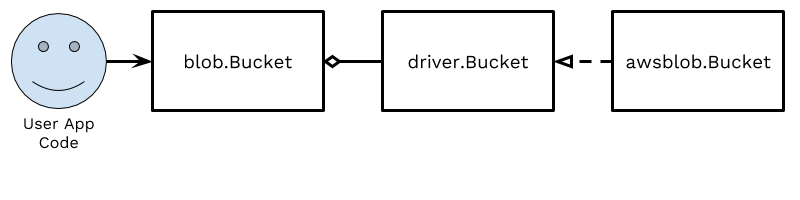
\includegraphics[scale=0.5]{Pictures/3_go_cdk.png}
    \caption{Go CDK API architecture.}
    \label{fig:3_go_cdk}
\end{figure}

This approach offers several advantages:
\begin{itemize}
    \item The portable type can handle complex logic internally, simplifying the driver's interface.
          For example, in the blob service, the NewWriter method of the portable type can determine the
          content type before interacting with the driver.
    \item It allows for the addition of new methods to the portable type without affecting backward
          compatibility, unlike modifying an interface which would be a breaking change.
    \item The portable type can seamlessly integrate new operations introduced in the driver through
          optional interfaces, eliminating the need for the user to perform type assertions.
\end{itemize}

\subsection{GORM}
GORM\textsuperscript{\cite{tech_12}} is a prominent ORM (Object-Relational Mapping) library for Go
(Golang), designed to be developer-friendly. It offers a full-featured ORM system with capabilities
such as associations (various relationship types), hooks (for create, save, update, delete, find
operations), and eager loading using Preload and Joins. GORM supports transactions, nested
transactions, context, prepared statement mode, and dry-run mode. It also provides functionality for
batch insert, SQL building, upserts, locking, and auto migrations. The library includes a logger,
extendable plugins, and is test-backed for each feature. Additionally, GORM supports composite
primary keys, indexes, and constraints, emphasizing its flexibility and developer-friendly nature.

\section{Serverless framework}
The Serverless Framework\textsuperscript{\cite{tech_13}} is a leading tool for deploying serverless
architectures. Developed after the release of AWS Lambda in 2014, it enables building applications
on cloud infrastructure that auto-scales and incurs no charges when idle. Key highlights include:

\begin{itemize}
    \item Empowering developers to focus more on building and less on managing.
    \item Supporting a wide range of serverless use-cases.
    \item Automated deployment of both code and infrastructure.
    \item Simple syntax for deploying AWS Lambda functions without needing in-depth cloud expertise.
    \item Multi-language support.
    \item Full lifecycle management of serverless architecture.
    \item Built-in support for multiple stages and environments.
    \item Extensibility through plugins.
\end{itemize}

The Framework streamlines serverless application development, offering tools for building,
deploying, updating, monitoring, and troubleshooting serverless architectures.

\subsection{Pros and cons}
The Serverless Framework offers a host of benefits for serverless architecture, such as facilitating
more efficient building with less management, supporting a wide range of use-cases, automating code
and infrastructure deployment, and providing simple syntax for safe AWS Lambda function deployment.
It supports multiple languages and manages the full lifecycle of serverless architecture,
accommodating large projects and teams with multi-domain and multi-environment support. The
framework is also highly extensible through its plugin ecosystem. However, it presents challenges
like a steep learning curve for newcomers, potential dependency issues, limited control over fine
infrastructure details, complexities in handling large-scale projects, and possible performance
bottlenecks. Also the variability in plugin reliability, the risk of vendor lock-in, and
challenges in cost management are significant considerations.

\subsection{Alternatives}

\begin{figure}
    \centering
    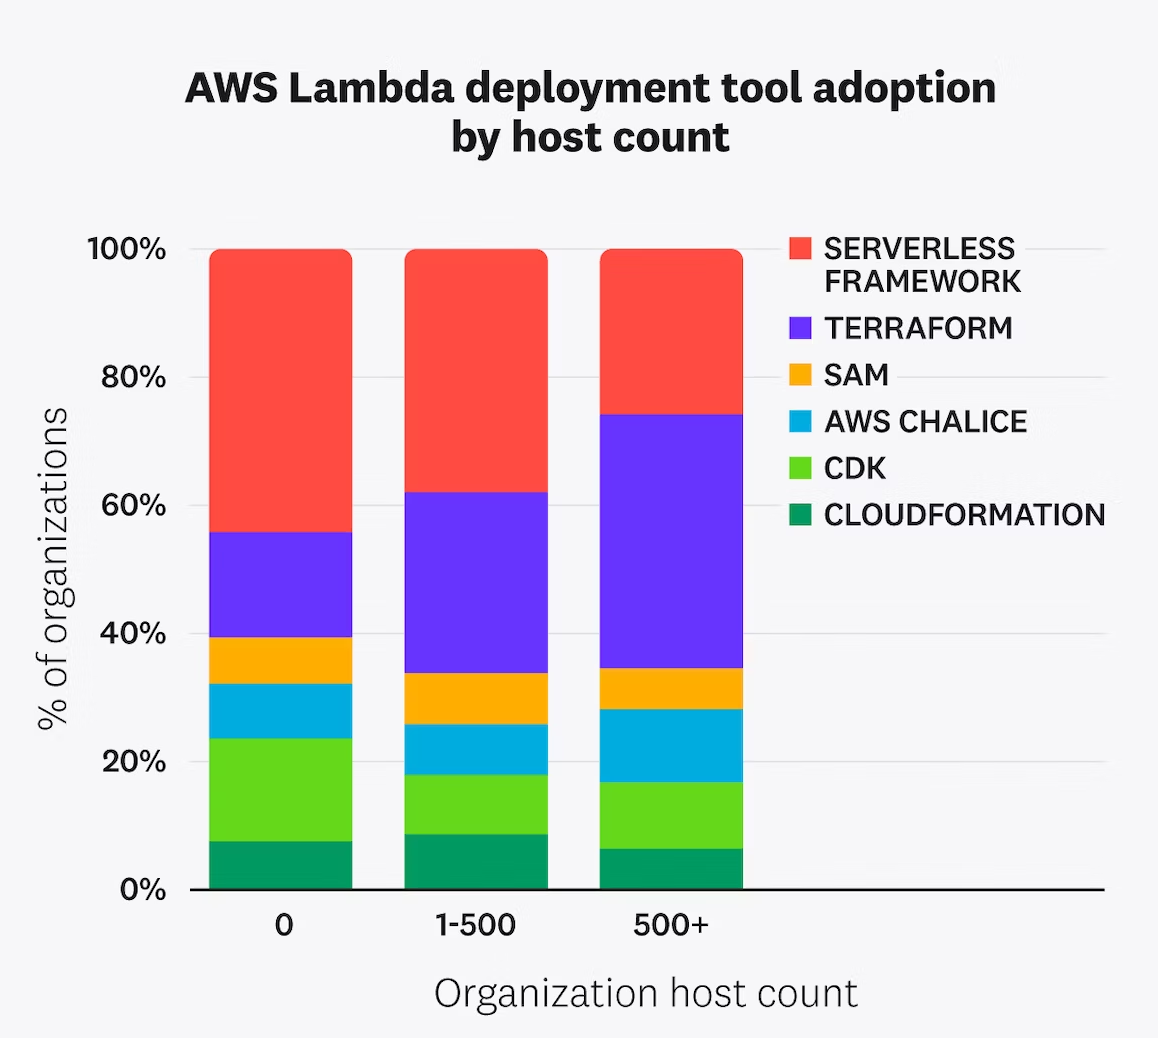
\includegraphics[scale=0.5]{Pictures/3_serverless_framework.png}
    \caption{Serverless Framework alternatives.}
    \label{fig:3_serverless_alternatives}
\end{figure}

Based on the image \ref{fig:3_serverless_alternatives} taken from a Datadog
research\textsuperscript{\cite{tech_14}}, it is evident that there are several alternatives to the
Serverless Framework for deploying functions, and their adoption varies according to the size of the
organization, measured by host count. In smaller companies with zero hosts, the Serverless Framework
is the clear frontrunner, indicating its preference among startups or for small-scale projects. For
mid-sized organizations, with host counts between 1 and 500, there is a more even split between the
Serverless Framework and Terraform, showing that both tools are well-suited for medium-scale
operations. However, in larger companies with over 500 hosts, Terraform emerges as the dominant
tool. This trend suggests that Terraform's versatility, its support for multiple cloud providers,
and its widespread adoption by DevOps teams make it the preferred choice for larger organizations
that likely have more complex and diverse cloud infrastructures.

\section{Flutter}
Flutter\textsuperscript{\cite{tech_15}} is an open-source UI software development kit created by
Google. It's used for building natively compiled applications for mobile, web, and desktop from a
single codebase. Flutter provides a fast development cycle with a "hot reload" feature that allows
instant updates without losing the state of the app. It offers expressive and flexible UI with a
rich set of widgets and a layered architecture that enables full customization. Flutter's native
performance is achieved through the use of Dart, which compiles to ARM or JavaScript code. This
toolkit is popular for its ability to create visually attractive and natively compiled applications
across platforms efficiently.

\subsection{Pros and cons}
Flutter, as a framework for app development, offers several compelling advantages alongside a few
drawbacks. Its ability to maintain consistency across multiple platforms with a single codebase
streamlines development, while the stateful hot reload feature significantly boosts developer
productivity. The framework's growing popularity is evident from its strong community support and
open-source nature, which fosters continual improvement and innovation. Flutter's approach to app
development with customizable widgets and excellent documentation facilitates faster and more
flexible app creation. However, being a relatively new entrant in the cross-platform arena, it faces
challenges such as limited learning resources, fewer plugins and packages compared to more
established frameworks, and larger app sizes due to its use of built-in widgets. Additionally, Dart,
the programming language for Flutter, has a smaller community, which might limit resources for
learning and development. These factors make Flutter a powerful but nuanced choice for app
developers, balancing its efficiency and ease of use against the considerations of newness and
community size.

\subsection{Architecture}
As depicted in figure \ref{fig:3_flutter_architecture}, Flutter is constructed as a modular, layered
framework. It comprises a set of autonomous libraries where each is built upon the layer beneath it.
There's no special access granted to any layer over the one it rests on, ensuring a democratic
structure. Additionally, the framework is engineered to be adaptable, with each segment crafted to
be optional and replaceable.

\begin{figure}
    \centering
    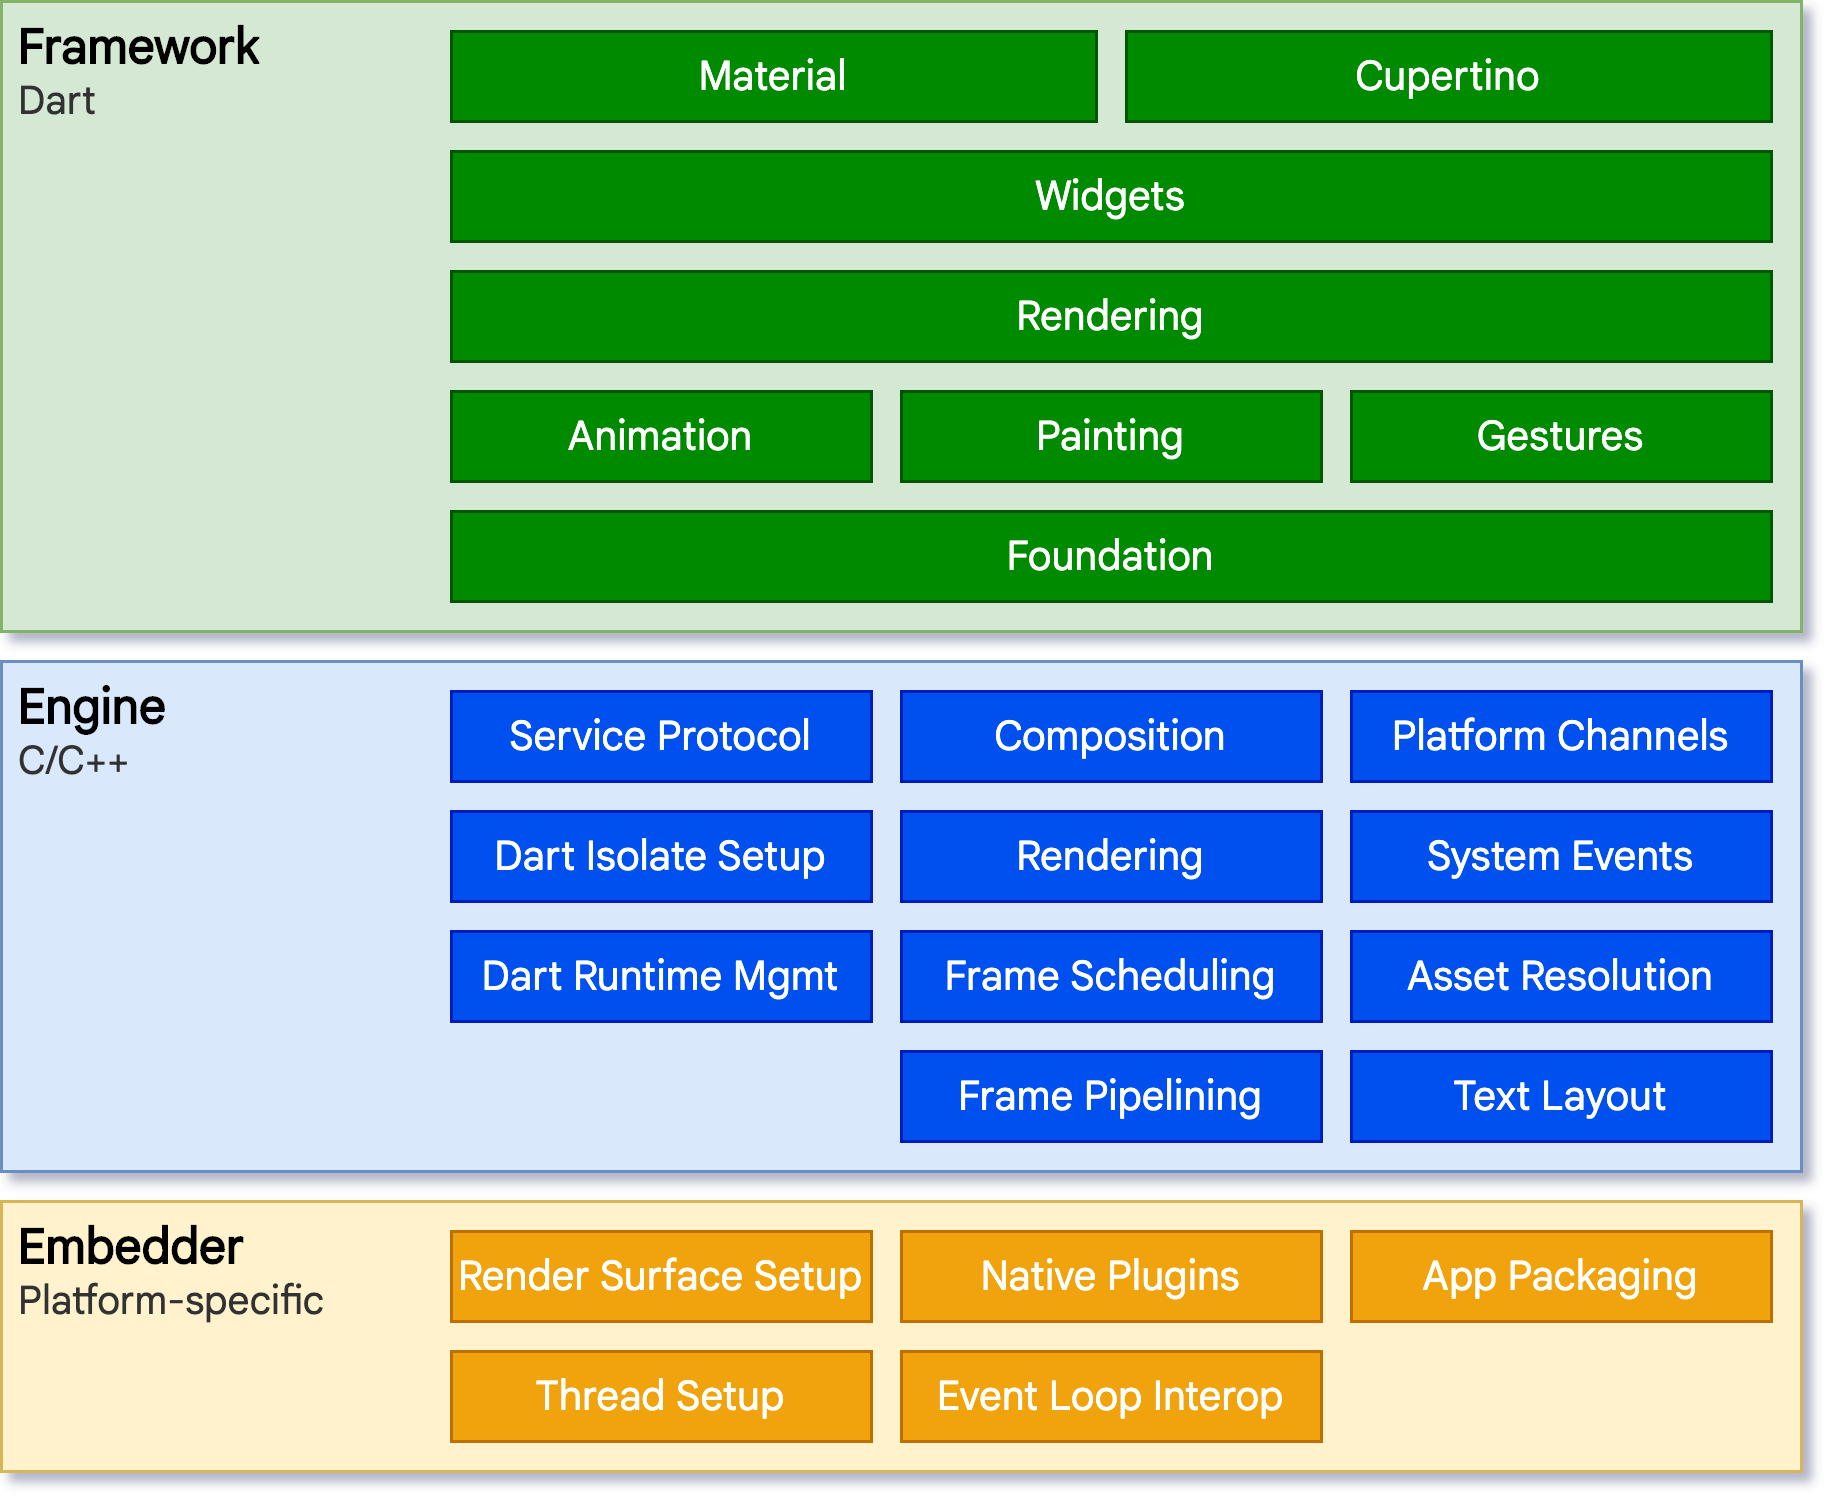
\includegraphics[scale=0.2]{Pictures/3_flutter.png}
    \caption{Flutter architecture.}
    \label{fig:3_flutter_architecture}
\end{figure}

To the base operating system, Flutter apps are wrapped and delivered just like any native app. The
platform-specific embedder acts as the initial entry point, interfacing with the OS for critical
services such as rendering surfaces, accessibility, inputs, and managing the messaging event loop.
This embedder layer is adaptable, written in the native languages of the platform such as Java and
C++ for Android, Objective-C/Objective-C++ for iOS and macOS, C++ for Windows and Linux, and
JavaScript for the web. Flutter's flexibility allows its code to be embedded within existing apps as
a module, or to form the entirety of a new application, supported by a variety of embedders tailored
for common target platforms, as well as third-party options.
\newline\newline
Central to Flutter's functionality is the engine layer, primarily crafted in C++. This engine
underpins every Flutter app by providing the essential components they require. It's tasked with
rasterizing composited scenes for painting new frames and underlies the core API of Flutter,
encompassing graphics (employing Impeller on iOS, soon on Android, and Skia elsewhere), text, file
and network I/O, accessibility, plugin infrastructure, and the Dart runtime with compilation tools.
\newline\newline
The bridge between the Flutter engine and the framework is dart:ui, which translates the engine's
C++ capabilities into Dart classes. This critical library introduces base primitives, enabling the
manipulation of input, graphics, and text rendering. Although the core Flutter framework is compact,
it is extendable, with numerous high-level functions available through additional packages, not
unlike the independent libraries stacked in the image, which collectively form the robust and
extensible framework that Flutter is known for.

\subsection{Alternatives}
Two major alternatives to Flutter for app development are React Native and Angular.
\newline\newline
React Native\textsuperscript{\cite{tech_16}}, developed by Facebook, is an open-source framework
tailored for building mobile applications. It allows developers to create natively rendered apps for
both iOS and Android using React, a popular JavaScript library. This framework embraces a 'learn
once, write anywhere' philosophy, enabling the use of a single codebase for multiple platforms while
retaining the capability to include platform-specific features. Known for its time and resource
efficiency, React Native can seamlessly integrate with existing native code, offering versatility in
development. It features live reloading for immediate reflection of code changes, boosting developer
productivity. With extensive community support, a wealth of libraries, and third-party plugin
compatibility, React Native is ideal for developers aiming for efficient cross-platform development
with a strong native performance and feel.
\newline\newline
Angular\textsuperscript{\cite{tech_17}}, developed by Google, is a comprehensive solution for web
application development. This platform and framework are geared towards building single-page client
applications using HTML and TypeScript. Angular streamlines the development and testing process with
tools for declarative templates, dependency injection, and integrated best practices. It features a
two-way data binding, reducing the need for additional code and enhancing efficiency for interactive
applications. Angular's architecture supports the rapid development of readable, maintainable, and
testable code, making it suitable for enterprise-level and complex web projects that demand
scalability and productivity. With its extensive libraries and strong community support, Angular is
an excellent choice for creating dynamic, high-performance web applications.
